\documentclass[prb,preprint]{revtex4-1} 
\raggedbottom
\usepackage{amsmath}
\usepackage{amsfonts}
\usepackage{graphicx}

\begin{document}

\title{Determination of the Half-Lives for \\ Isotopes of $^{108}$Ag, $^{110}$Ag, and $^{116m}$In}

\author{Ryan S. Morshead}

\affiliation{Department of Physics, California State Polytechnic University}

\date{\today}

\begin{abstract}

Using a Gieger tube to measure $\beta^-$ decays from the silver isotopes of $^{108}$Ag and $^{110}$Ag to $^{108}$Cd and $^{110}$Cd in order to determine their half-lives of the parent nuclei. To achieve the same result for the excited indium isotope of $^{116m}$In we use a scintillation crystal in combination with a photomultiplier tube to measure gamma radiation emitted during its decay to $^{116}$Sn. The count data produced was characterized using non-linear least squares optimizations of fit functions detailed later in the report. These optimized fit functions were used to calculated half-lives. Using this method we find the half-lives of $^{108}$Ag, $^{110}$Ag, and $^{116m}$In to be $170\pm30$ s, $31\pm2$ s, and $51.0\pm0.3$ min respectively. The result for $^{108}$Ag is in agreement with the accepted value of 142.2 s while our value for $^{110}$Ag is in disagreement with the accepted value of 24.6 s\cite{dat}. Our value for $^{116m}$In is in disagreement with the accepted value of 54.29 min\cite{dat}.


\end{abstract}


\maketitle


\section{Introduction}

When the French physicist Henri Becquerel discovered what he called uranium rays in 1896 and when Marie Curie began to study them, one of the givens of physical science was that the atom was indivisible and unchangeable\cite{curie,henri}. The work of Becquerel and Curie soon led other scientists to suspect that this theory of the atom was not sustainable.

Scientists soon learned that some of the mysterious ``rays" emanating from radioactive substances were not rays at all, but tiny particles \cite{ernest}. The surprising things was that radioactivity was no more nor less than the emission of tiny particles and energetic waves from the atom. Building on the research of Marie Curie and others, scientists soon realized that if atoms emitted such things they could not be indivisible and unchangeable. Atoms are made up of smaller particles, and these can be rearranged.

In 1900 Ernest Rutherford found that the radioactivity of the ``emanation" (as he called it) from thorium diminished with time\cite{eminations}. This decay of radioactivity was a vital to making further progress. Rutherford, while working in Canada with the chemist Frederick Soddy, developed a revolutionary hypothesis to explain the process. They realized that radioactive elements can spontaneously change into other elements\cite{es}. As they do so, they emit radiation of one type or another. The spontaneous decay process continues in a chain of emissions until a stable atom is formed. It was, as Rutherford and Soddy boasted, the transmutation of elements that had eluded alchemists for thousands of years\cite{es}. They recognized at once that the ceaseless emissions pointed to a vast store of energy within atoms\cite{es}.

The objective of this report is to make calculations of half-lives, which characterize atomic decay rates, for the unstable isotopes of $^{108}$Ag, $^{110}$Ag, and an excited state of $^{116}$In, $^{116m}$In.

\newpage

\section{Experimental Design}

We begin by exposing thin foils of silver, which contain isotopes of $^{107}$Ag and $^{109}$Ag, along with foils of $^{115}$In, to a strong neutron emitter. In this case we expose them to a radioactive combination of plutonium and beryllium which has a decay rate of approximately 3 Ci. In the presence of this emitter the foils become radioactive after capturing additional neutrons; where $^{107}$Ag and $^{109}$Ag activate to $^{108}$Ag and $^{110}$Ag respectively while $^{115}$In activates to $^{116}$In and an excited state of $^{116m}$In. The half-lives of the activated isotopes are $\approx2.5$ min, $\approx30$ s, $\approx1$ hr, and $\approx14$ s respectively. We then determine how long the foils of aluminum and indium must be exposed to the neutron emitter in order to conduct our experiment. This is done by assuming that the rate of neutron accruement is constant while the rate at which the newly formed radioactive isotopes decay is dependent on the number of isotopes present. With these assumptions we build the expression
\begin{equation}\label{daccruement}
dN/dt=p-AN,
\end{equation}
where $N$ is the number of radioactive isotopes present in the foil, $p$ is the rate of neutron accruement, and A is the probability that a nucleus will decay. By substituting in $\tau$ and integrating this equation we find 
\begin{equation}\label{accruement}
N(t_r)=\frac{p}{A}\left(1-e^{-t_r/\tau}\right),
\end{equation}
where $t_r$ is the irradiation time and $1/A=\tau$, the time required for the initial population to be reduced by a factor of $e^{-1}$. Through Eq \eqref{accruement} we see that for large values of $t_r$, $N$ approaches $p/A$ the maximum neutron accruement $N_{max}$. Thus $N_{max}=p/A$. For our purposes we choose $t_r\approx5T_{1/2}$ where the half-life, $T_{1/2}$, equals $\tau ln(2)$. As such about $97\%$ of the original material will be activated. Using this value for $t_r$ we find that the silver foil can be activated in $\approx15$ mins while indium takes $\approx5$ hrs.

The two silver isotopes produced after irradiation undergo a $\beta^-$ decay to cadmium. because the majority of the decays to cadmium do so to an unexcited state ($\approx97\%$ in $^{108}$Ag and $\approx94\%$ in $^{110}$Ag) there is very little gamma radiation. We choose to measure silver's $\beta^-$ decays with a Geiger tube for this reason. The decay schemes for $^{108}$Ag and $^{110}$Ag are shown in Fig. \ref{Ag_scheme}.

\begin{figure}[h!]
\centering
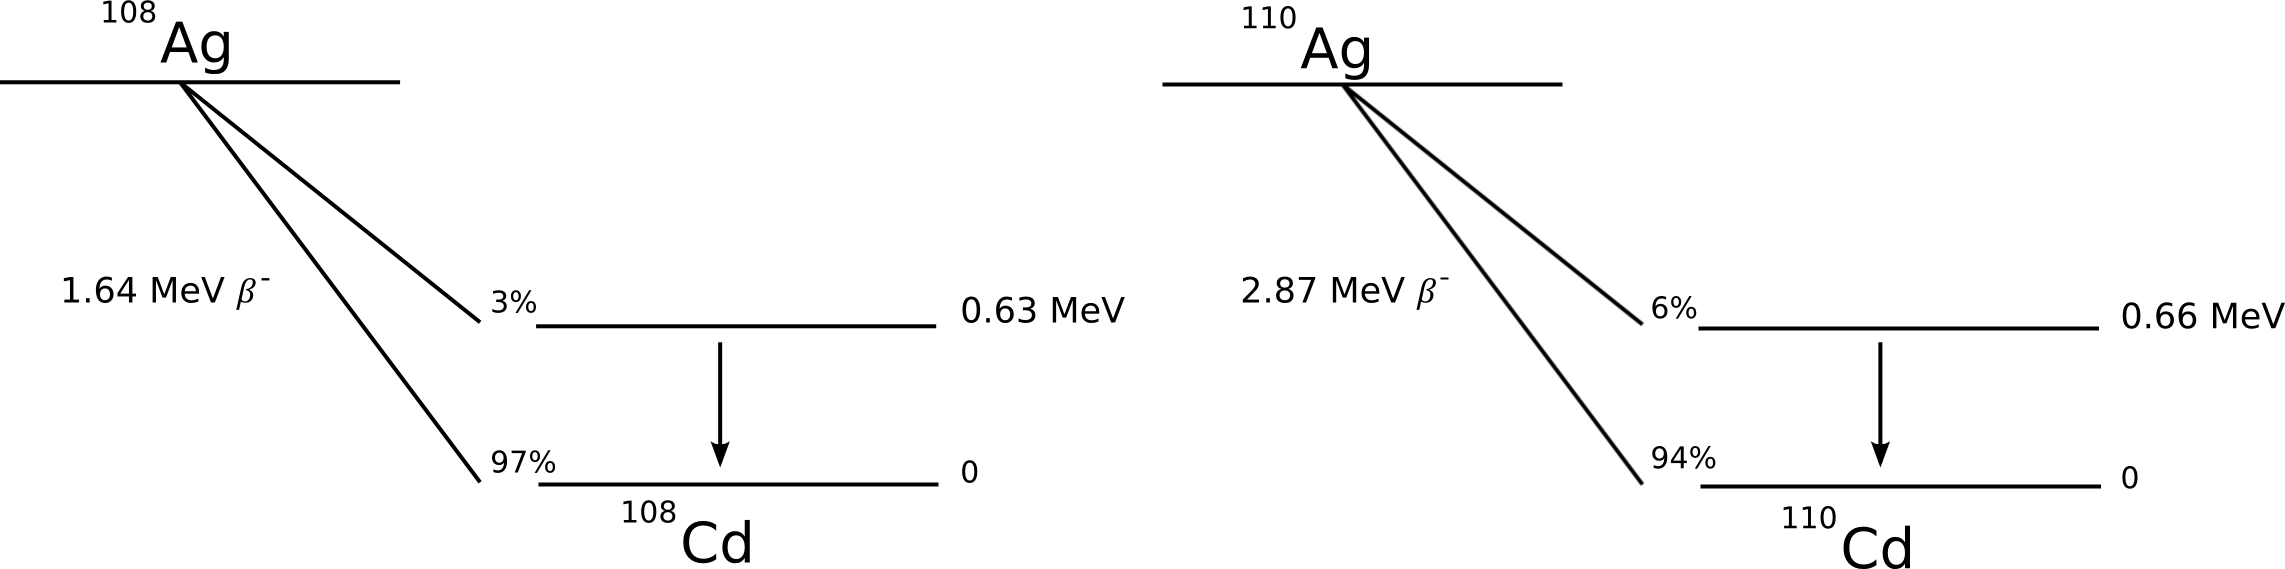
\includegraphics[scale=.26]{DecayScheme.png}
\caption{Decay scheme for $^{108}$Ag to $^{108}$Cd and for $^{110}$Ag to $^{110}$Cd}
\label{Ag_scheme}
\end{figure}

\newpage

The indium isotope produced after irradiation can be found in an excited state and in a ground state. Since the ground state has a half-life of about $14$ s, making it very difficult to evaluate, we instead measure gamma radiation from $^{116m}$In who's half-life is significantly longer. This excited sate of indium then decays to tin in various excited states which release cascades of gamma rays upon returning to the ground state. The decay scheme for indium is shown in Fig \ref{In_scheme}. To measure the radiation from indium we choose to use a scintillation detector because of the efficiency with which it measures gamma radiation. 

\begin{figure}[h!]
\centering
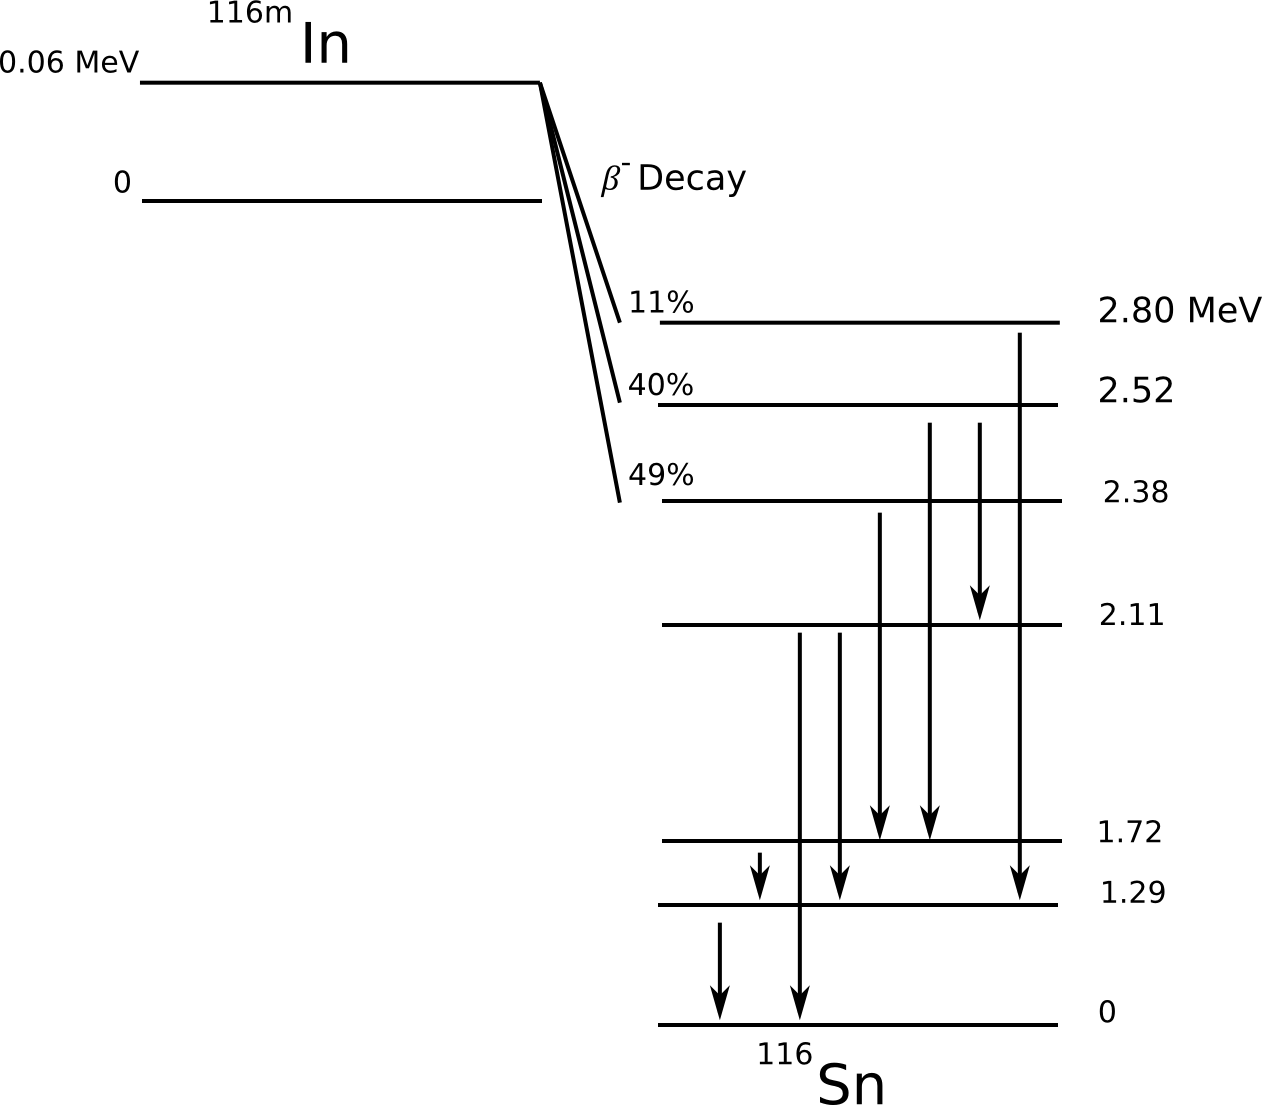
\includegraphics[scale=.26]{DecayScheme1.png}
\caption{Decay scheme for $^{116m}$In to $^{116}$Sn}
\label{In_scheme}
\end{figure}

\newpage

To describe the transitions of cadmium and tin from their excited states we use reasoning similar to what was used in Eq \eqref{daccruement} to produce the equation
\begin{equation}\label{dexcited}
dN/dt=-AN,
\end{equation}
where $N$ now represents the number of excited atoms present at a time $t$ and A represents the probability of a transitioning to a lower energy state. This expression notably lacks and accruement term as our measurements will not be taken in the presence of a neutron emitter. We then solve this differential equation producing the expression
\begin{equation}\label{excited}
N(t)=N_0e^{-t/\tau},
\end{equation}
Where $N_0$ is the initial amount of amount of atoms present. However we are not able to measure the number of atoms present at any particular time, instead we count some fraction of decays over a specific time interval. As such we are analogously measuring some fraction $f$ of the true decay rate $R$ at a particular time $t$. To relate Eq \eqref{excited} to R which is equivalent to $dN/dt$ we can say that $R(t)=AN$. Because we know $N$ from Eq \eqref{excited} we can then produce the expression
\begin{equation}\label{Rexcited}
R(t)=AN_0e^{-t/\tau},
\end{equation}
where we know $AN_0$ to be the initial decay rate. Then because we don't measure all decays we must include $f$ to produce the count rate $R_c$. With this, $R_c(t)=fR(t)$, producing the final expression
\begin{equation}\label{Rmexcited}
R_c(t)=R_0e^{-t/\tau},
\end{equation}
where $fAN_0=R_0$, the initial count rate.

For measuring silver decays we use a Geiger tube which is attached to a preamp, amplifier, multichannel analyzer (MCA), and oscilloscope as shown in Fig \ref{ExpFig1}. To take valid measurements the voltage supplied to the geiger tube must in the plateau region, for this reason we choose that voltage to be 850 V. We then adjust the amplifier gain such that pulses produced by a $^{137}$Cs source are register between 1 and 2 V and utilize the multichannel scaler mode on the MCA with a dwell time, $\Delta t$, of 2.5 s.

The multichannel scaler mode uses the 256 channels in the MCA as sequential counters. As such each channel individually measures counts over $\Delta t$ switching from one channel to the next after each completed measurement. Knowing that the number of counts, $C(t)$ is equivalent to $R_c(t)\Delta t$ we can rewrite Eq \eqref{Rmexcited} as
\begin{equation}\label{Cexcited}
C(t)=C_0e^{-t/\tau}.
\end{equation}
by dividing through by $\Delta t$. In this context we then find that the measurement on the first channel will be equivalent to $C_0$ and that the time of this measurement will be zero showing that we can easily relate our measurements to . We say this because Eq \eqref{Cexcited} is relevant no matter what time is considered to be zero. With this we can then say that the time associated with any particular measurement will be $(n-1)\Delta t$ where n is the channel number starting from one.

\begin{figure}[h!]
\centering
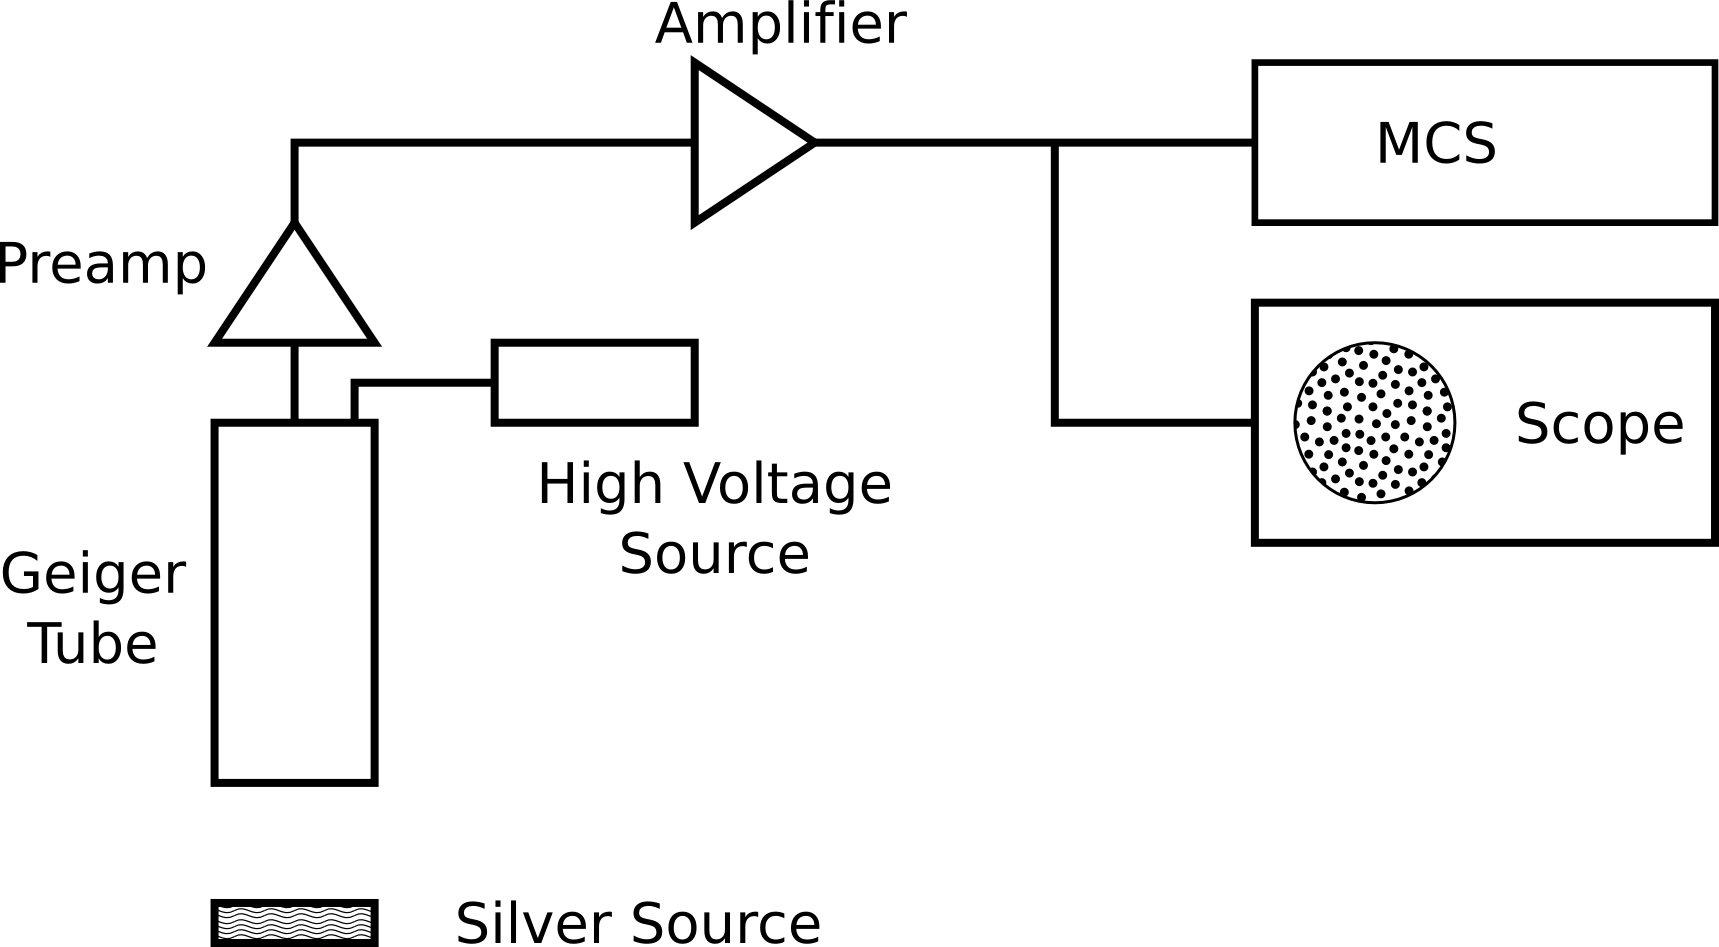
\includegraphics[scale=.2]{ExpFig_silver.png}
\caption{Experimental setup for a silver source}
\label{ExpFig1}
\end{figure}

For measuring Indium decays we send the amplified pulses produced by the scintillator and photomultiplier tube through a single channel analyzer (SCA) as shown in Fig \ref{ExpFig2}. Here we use a comparator circuit to compare the heights of the pulses against a preset voltage called the discriminator level. If pulse heights fall below the discriminator level they are discarded, but those that do not are recorded.

\begin{figure}[h!]
\centering
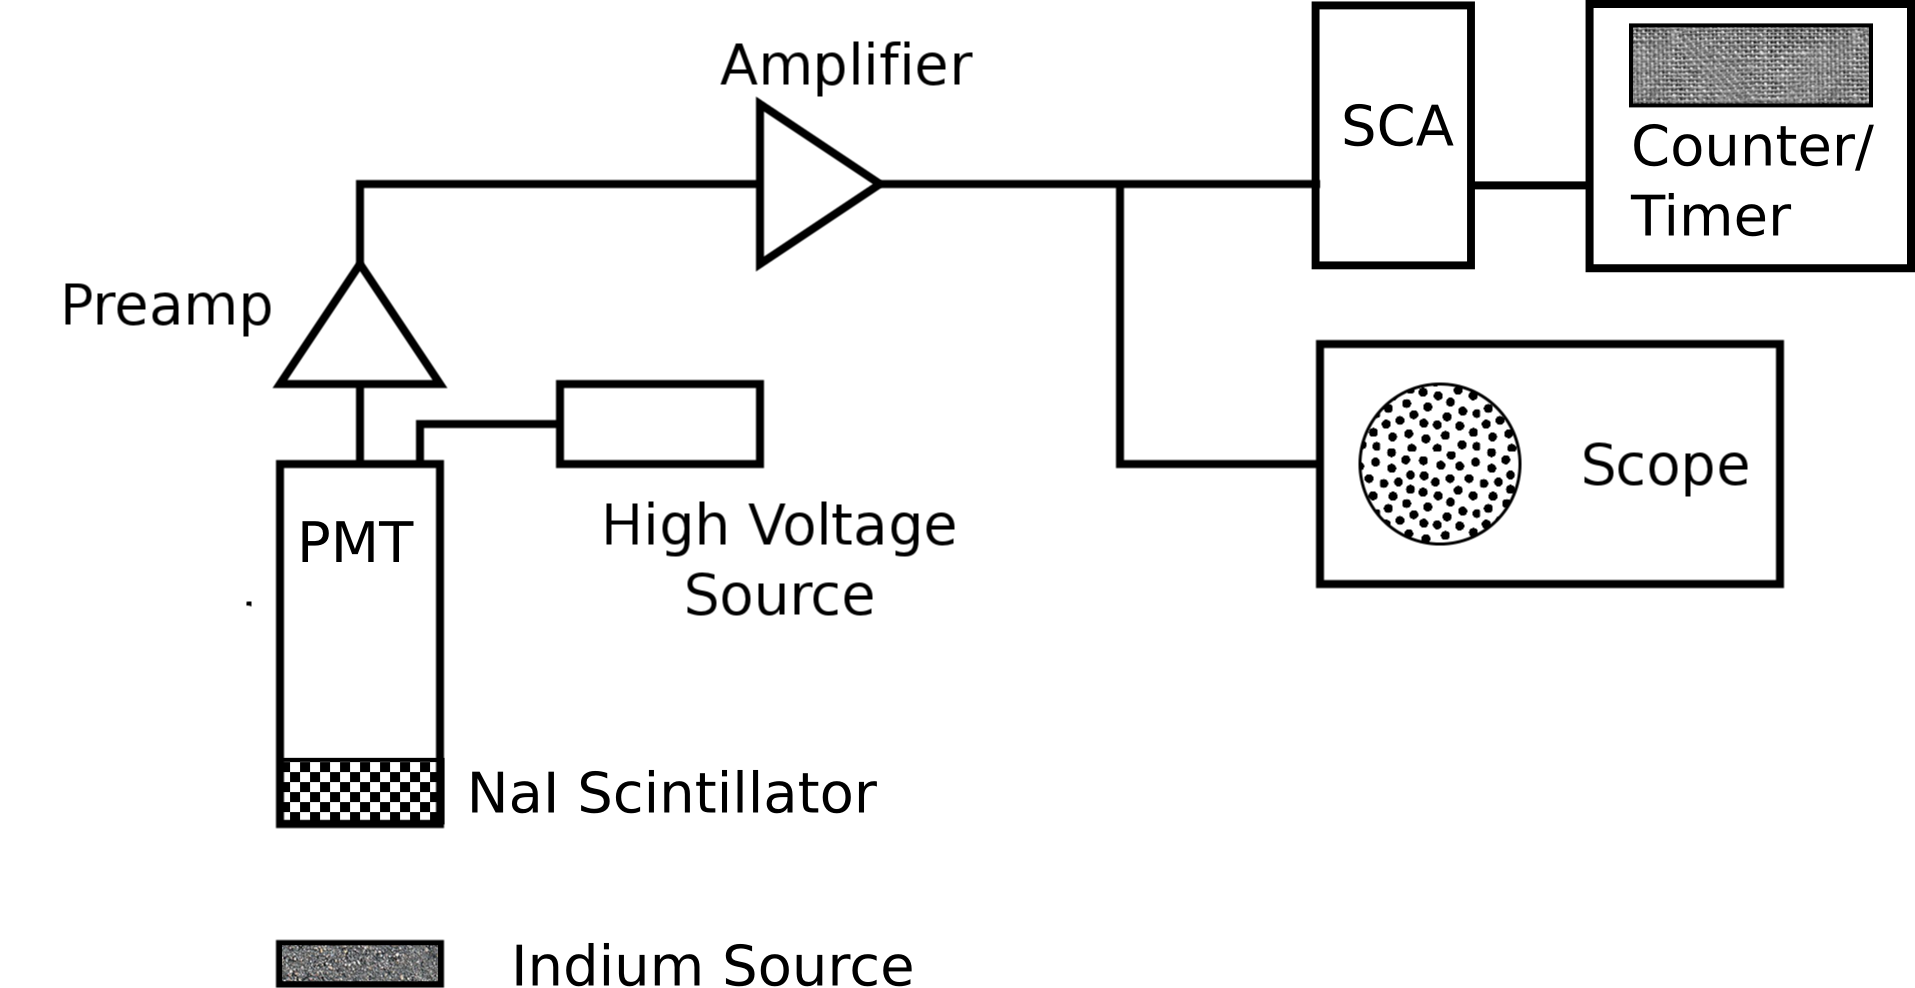
\includegraphics[scale=.2]{ExpFig_indium.png}
\caption{Experimental setup for an indium source}
\label{ExpFig2}
\end{figure}

To analyze the data collected from the silver source we must make a correction due to the excess charge created at the anode after each photon incident on the walls of the Geiger tube. The period of time the tube suppresses pulses which would normally be created by photons striking the tube is called the dead time, $\tau_d$. To characterize the true number of counts which would be recorded absent any dead time, we devise the following expression:
\begin{equation}\label{ctrue}
C_{true}=\frac{C_{obs}}{1-\tau_d (C_{obs}/t_i)}.
\end{equation}
This is formulated under the assumption that there is a fraction of electrons $\tau_d (C_{obs}/t_i)$ which will not be recorded by the tube, where $C_{true}$ is the correct number of counts, $C_{obs}$ is the observed number of counts, and $t_i$ is the integration time for each measurement. Note that we choose $t_i$ to be 4 seconds, making the observed count rate equal to $C_{obs}/4$.

With corrected count data we must be aware that our data is a reflection of three things; decays associated with the short lived isotope of $^{110}$Ag, decays associated with the more enduring $^{108}$Ag, and background counts. With this knowledge we must conclude that our data can be modeled with a function of the form
\begin{equation}\label{fit}
f(t)=Ae^{-t/\tau_1}+Be^{-t/\tau_2}+C,
\end{equation}
where we include a constant background term $C$, and two terms of the form of Eq \eqref{Cexcited} with each being representative of one kind of silver decay. As such $A$ and $\tau_1$ are characteristic of one decay while $B$ and $\tau_2$ are characteristic of the other. In order to fit this function to the data we first use a weighted non-linear least squares optimization of $B$, $\tau_2$, and $C$. To do this, we choose $Ae^{-t/\tau_1}$ to be associated with decays from $^{110}$Ag, and $Be^{-t/\tau_2}$ with decays from $^{108}$Ag. Using this we can say that after some period of time, $t_a$, we can approximate $Ae^{-t/\tau_1}$ to be 0. We can then apply our least squares optimization of $f(t)$ to data after $t_a$ thereby determining $B$, $\tau_2$, and $C$. With this we make yet another non-linear least squares optimization of the remaining unknown values in $f(t)$ to all the data thereby solving for $A$ and $\tau_1$. With $\tau_1$ and $\tau_2$ known we can then determine the half-lives of the two silver isotopes.

To analyze data collected from the indium source we must subtract off background counts. However to determine background counts, instead of conducting integrations without a source present we instead choose to use an inactive $^{115}$In as the source. This is done because $^{115}$In has a half-life, and by making it a source in background measurements the rate of its undesired beta decays are determined in addition to any other count sources present. We take background counts prior to, and following data acquisition, averaging the two and subtracting that value from our recorded source counts to determine the net counts, $C_{net}$. At the point where $C_{net}$ becomes negative and the measured values are lost in the background we ignore all subsequent data points. Then, by taking the natural log of $C_{net}$ and relevant fit function, Eq \eqref{Cexcited}, we linearize our data and fit function. Using $ln(C_{net})$ values and the natural log of Eq \eqref{Cexcited}, which is
\begin{equation}\label{log_fit}
ln(C(t))=ln(C_0)-t/\tau,
\end{equation}
a weighted linear least squares optimization of $C_0$ and $\tau$ is performed to fit the data. With the optimized value for $\tau$ we can then determine the half-life of $^{116m}$In.

\section{Results and Analysis}
\subsection{Silver}
Here we have two sets of data which are shown in Fig \ref{Silver} and Fig \ref{Silver_log}, however we only provide analysis on one set. This is because a software issue in our dwell time. The initial setting for Trial 1 used a dwell time of 4 s which resulted in a true dwell time of 1 s.  With 1 second integration times on each channel we had at most 256 seconds of data to measure a half life which was close to half that. In order to get a good measurement of the half-life, one would need $\approx$5 half-lives of data collection. As such the longer-lived silver isotope with a half life of $\approx$2.5 min requires $\approx$750 seconds worth of data. To perform analysis we use a second set of data which uses a set dwell time of 10 s and true dwell time of 2.5 seconds making our total time collection time 640 s. This gives a significant improvement over our initial calculations. Fig \ref{Silver}, more so than Fig \ref{Silver_log}, demonstrates visually with data that has been scaled down by a factor of 100 the inability of our first trial to represent the true decay trend shown by Trial 2. With this increased time interval on our second trial we are capable of using a $t_a$ of 300 s which is greater than $12T_{1/2}$ for $^{110}$Ag. At 300 s the count rate for $^{110}$Ag is $\ll1\%$ of its initial rate while $^{108}$Ag maintains a count rate which is $\approx13\%$ of its initial rate. With this value of $t_a$ we are capable of measuring $^{108}$Ag decays and approximating the rate of $^{110}$Ag decays to be 0 in our first non-linear least squares fit. The results of the non-linear least squares optimizations detailed previously produced values for $\tau_1$ and $\tau_2$ which are $44\pm9$ s and $240\pm40$ s respectively. The half-lives which are produced are then $170\pm30$ s for $^{108}$Ag and $31\pm2$ s for $^{110}$Ag. The result for $^{108}$Ag is in agreement with the accepted value of 142.2 s while our value for $^{110}$Ag is in disagreement with the accepted value of 24.6 seconds\cite{dat}. 
\begin{figure}[h!]
\centering
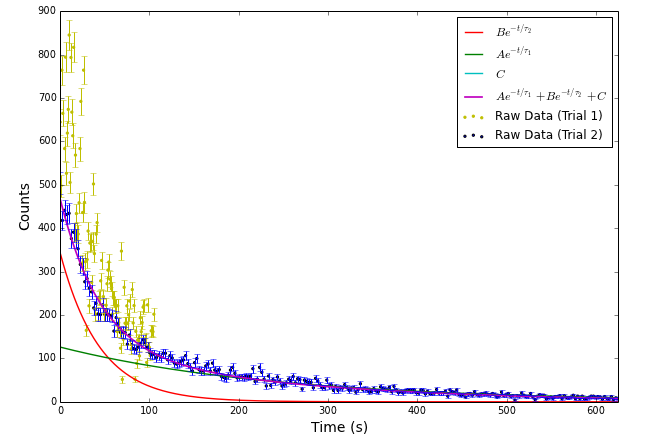
\includegraphics[width=.75\textwidth]{Silver.png}
\caption{Data from Trial 1 which is }
\label{Silver}
\end{figure}

\begin{figure}[h!]
\centering
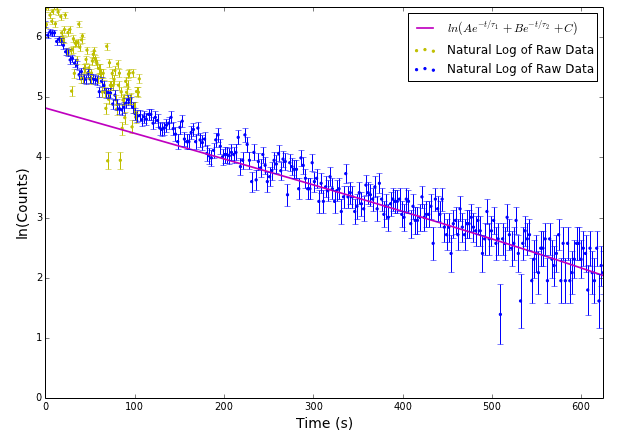
\includegraphics[width=.71\textwidth]{Silver_log.png}
\caption{Experimental setup for an indium source}
\label{Silver_log}
\end{figure}

\newpage

\subsection{Indium}
The half-life of indium was determined using a non-linear least squares optimization of Eq \eqref{log_fit} based on the data shown in Fig \ref{Indium}. This optimization determined $\tau$ to be $73.5\pm0.4$ min thereby showing $T_{1/2}$ to be $51.0\pm0.3$ min. Our value for $^{116m}$In is in disagreement with the accepted value of 54.29 min\cite{dat}.

\begin{figure}[h!]
\centering
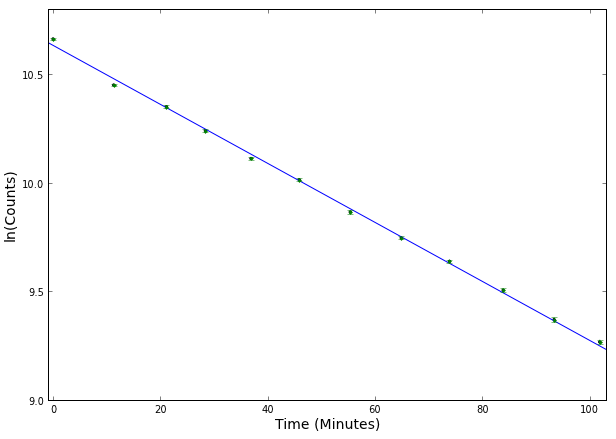
\includegraphics[width=.75\textwidth]{Indium.png}
\caption{Experimental setup for an indium source}
\label{Indium}
\end{figure}

\newpage

\section{Conclusion}

Though some results do not agree with their corresponding accepted values, the objective of this result was achieved with the measurement of the half-lives of $^{108}$Ag, $^{110}$Ag, and $^{116m}$In. As previously described the count data gathered and characterized using non-linear least squares optimizations of fit functions as described in section III. These optimized fit functions were used to calculated half-lives. By this method we find that the half-lives of $^{108}$Ag, $^{110}$Ag, and $^{116m}$In are $170\pm30$ s, $31\pm2$ s, and $51.0\pm0.3$ min respectively. The result for $^{108}$Ag is in agreement with the accepted value of 142.2 s while our value for $^{110}$Ag is in disagreement with the accepted value of 24.6 s\cite{dat}. Our value for $^{116m}$In is in disagreement with the accepted value of 54.29 min\cite{dat}.

\newpage

\begin{acknowledgments}

asdasdasdasd

\end{acknowledgments}


\begin{thebibliography}{99}

\bibitem{henri} Henri Becquerel (1896). ``Sur les radiations �mises par phosphorescence". Comptes Rendus \textbf{122}: 420--421.

\bibitem{curie} Mould, R. F. (1998). ``The discovery of radium in 1898 by Maria Sklodowska-Curie (1867--1934) and Pierre Curie (1859--1906) with commentary on their life and times". The British Journal of Radiology \textbf{71} (852): 1229--54.

\bibitem{ernest} Ernest Rutherford (1911). The scattering of alpha and beta particles by matter and the structure of the atom. Taylor \& Francis: 688.

\bibitem{eminations} E. Rutherford, ``Emanations from Radio-active Substances,'' Nature, \textbf{1901}, \textit{64}, 157.

\bibitem{es} Philosophical Magazine 4, 370-96 (1902) The Collected Papers of Lord Rutherford of Nelson, Vol. 1, pp. 472-94. London: Allen and Unwin, Ltd.

\bibitem{dat} Firestone, Richard B. ``The Berkely Laboratory Isotopes Project" \\http://ie.lbl.gov/education parent/In\_iso.html (accessed on Dec 5, 2013)

\end{thebibliography}

\end{document}
